\documentclass[12pt,letterpaper]{article}
\usepackage[margin=1.5in]{geometry}
\usepackage[T1]{fontenc}
\usepackage[utf8]{inputenc}
\usepackage[spanish,es-nodecimaldot]{babel}
\usepackage{mathpazo}
\usepackage{microtype}
\usepackage{amsmath,amssymb,amsfonts,bm}
\usepackage{graphicx}
\usepackage{tabularx}
\usepackage{subfig}
\usepackage{booktabs}
\usepackage{xcolor}
\usepackage[colorlinks=true,linkcolor=black,citecolor=black,urlcolor=blue]{hyperref}
\usepackage{eurosym}
\newcommand{\e}{\mathrm{e}}

\title{\textbf{Incentivos y estructura organizativa en la financiaci\'on hospitalaria}}
\author{Jose Mar\'\{\i\}a Elena-Izquierdo}
\date{}

\begin{document}
\maketitle

\begin{abstract}
La financiaci\'on eficiente de los hospitales no depende solo de las f\'ormulas de pago, sino tambi\'en de las relaciones organizativas entre los agentes que participan en la prestaci\'on asistencial. Este trabajo estudia c\'omo distintas estructuras organizativas condicionan el uso \'optimo de incentivos para directivos hospitalarios y m\'edicos en presencia de riesgo moral. Desarrollamos un modelo de m\'ultiples tareas con dos niveles de contrataci\'on y caracterizamos la soluci\'on de segundo \'optimo bajo contrataci\'on centralizada y descentralizada. Las simulaciones num\'ericas muestran c\'omo el ruido en las se\~nales de desempe\~no y el grado de complementariedad o sustituibilidad entre tareas afectan tanto a la intensidad \'optima de los incentivos como a los niveles de esfuerzo de equilibrio.
\end{abstract}

\section*{Introducci\'on}
La atenci\'on hospitalaria es el resultado de la interacci\'on de m\'ultiples agentes. Los financiadores, p\'ublicos o privados, compran servicios a los hospitales. Los directivos hospitalarios asignan recursos humanos y materiales. Dentro del hospital, m\'edicos, enfermeras, auxiliares, farmac\'euticos y otros profesionales desarrollan tareas diferenciadas cuyos esfuerzos conjuntos determinan diagn\'osticos, tratamientos y, en \'ultima instancia, resultados en salud.

Esta multiplicidad de agentes y tareas tiene implicaciones directas para la financiaci\'on hospitalaria. El primer objetivo de este trabajo es, por tanto, modelizar la naturaleza multiagente y multitarea de la actividad hospitalaria. Un punto de partida natural es la literatura sobre riesgo moral bilateral en salud, en la que tanto hospitales como m\'edicos influyen en el desempe\~no y el dise\~no contractual debe tener en cuenta esa interdependencia estrat\'egica.

Un segundo objetivo es incorporar el entorno institucional en el que se aplican esos contratos. En el caso espa\~nol, los hospitales p\'ublicos siguen siendo la forma organizativa dominante, aunque en las \'ultimas d\'ecadas han ganado peso proveedores privados, entidades sin \'animo de lucro y partenariados p\'ublico-privados. M\'as all\'a de la titularidad jur\'idica, una diferencia relevante es el grado de autonom\'ia directiva. En buena parte del sistema p\'ublico, las autoridades sanitarias regionales contratan los servicios y el personal mediante procedimientos relativamente centralizados. En cambio, los hospitales privados y no lucrativos suelen disponer de mayor discrecionalidad para configurar plantillas y dise\~nar la remuneraci\'on de los m\'edicos. En esos entornos son m\'as frecuentes los pagos variables y la retribuci\'on ligada a actividad, mientras que en el sector p\'ublico predominan los salarios fijos complementados con incentivos de menor intensidad.

El modelo que se desarrolla a continuaci\'on incorpora estas alternativas organizativas. Analizamos c\'omo cambian las restricciones de compatibilidad de incentivos cuando el financiador contrata simult\'aneamente con el hospital y con el m\'edico, frente a una estructura descentralizada en la que el financiador solo contrata con el hospital y este dise\~na la remuneraci\'on del m\'edico. El objetivo es obtener implicaciones sobre la intensidad \'optima de los incentivos y sobre la eficiencia productiva en un entorno multiagente y multitarea con riesgo moral. En t\'erminos m\'as amplios, se pretende derivar resultados contrastables emp\'iricamente en el sistema hospitalario espa\~nol.

\section{El modelo}

\subsection{Planteamiento}
En el modelo interact\'uan tres agentes: el comprador de servicios sanitarios, que puede ser p\'ublico o privado; la direcci\'on del hospital, a la que nos referiremos simplemente como el hospital; y el m\'edico. Hospital y m\'edico producen conjuntamente dos outputs. El primero es la cantidad de servicios, interpretada por ejemplo como el n\'umero de ingresos:
\begin{equation*}\label{eq:qes}
  q(a,t_1)=a+t_1+\epsilon_1
\end{equation*}
La variable no negativa $a$ representa el esfuerzo del hospital destinado a aumentar el volumen asistencial, mientras que $t_1$ es el esfuerzo del m\'edico orientado a esa misma dimensi\'on. El output depende de ambos esfuerzos y de una perturbaci\'on aleatoria $\epsilon_1$.

El segundo output es la intensidad, utilizada aqu\'i como aproximaci\'on a la calidad.\footnote{La calidad es un concepto dif\'icil de definir en el entorno hospitalario. Por simplicidad, el modelo se centra en la intensidad asistencial por paciente.} Esta dimensi\'on depende del esfuerzo del m\'edico $t_2$ y de una perturbaci\'on aleatoria $\epsilon_2$:
\begin{equation*}\label{eq:ies}
  i(t_2)=t_2+\epsilon_2
\end{equation*}
Se supone que el hospital puede influir en el n\'umero de altas, pero no en la cantidad de servicios diagn\'osticos o terap\'euticos por paciente, una decisi\'on que recae exclusivamente en el m\'edico.

El vector de outputs es $\bm{x}=(q,i)$. Los t\'erminos aleatorios son $\bm{\epsilon}=(\epsilon_1,\epsilon_2)$, distribuidos normalmente con media cero y matriz de varianzas-covarianzas
\[
\Sigma=
\begin{pmatrix}
\sigma_1^2 & \sigma_{12}^2 \\
\sigma_{12}^2 & \sigma_2^2
\end{pmatrix},
\qquad
\bm{\epsilon}\sim N(\mathbf{0},\Sigma).
\]

Las utilidades de los tres agentes son:
\begin{eqnarray*}\label{utiles}
u_f &=& s(q,i)-\lambda[b(q,i)+w(q,i)]\\
u_h(b,a) &=& u_h[b(q,i)-\tau(a)+z(a)]\\
u_m(w,t_1,t_2) &=& u_m[w(q,i)-\psi(t_1,t_2)+\phi(t_1,t_2)]
\end{eqnarray*}
donde $s(q,i)$ es el beneficio bruto del financiador, $b(q,i)$ es el pago al hospital y $w(q,i)$ es la remuneraci\'on del m\'edico. Hospital y m\'edico soportan costes de esfuerzo recogidos por $\tau(a)$ y $\psi(t_1,t_2)$, respectivamente. Adem\'as, permitimos motivaciones altruistas o vocacionales, representadas por $z(a)$ para el hospital y $\phi(t_1,t_2)$ para el m\'edico.

\subsection{El primer mejor}
Bajo informaci\'on completa, el principal observa los esfuerzos de ambos agentes y contrata bajo una estructura centralizada.\footnote{Con informaci\'on completa, una estructura descentralizada implementa los mismos niveles de esfuerzo de primer mejor, por lo que basta con utilizar el caso centralizado como referencia.} El problema del principal es:
\begin{eqnarray*}\label{maxf0es}
\nonumber \max\limits_{a,t_1,t_2}\,
\mathbb{E}_{\bm{\epsilon}}[u_f]
&=&
\mathbb{E}_{\bm{\epsilon}}
\left[
s(q(.),i(.))-\lambda\big(b(q(.),i(.))+w(q(.),i(.))\big)
\right]\\
\nonumber \text{sujeto a }\\
\mathbb{E}_{\bm{\epsilon}}[u_h] &\geq& u_h(\bar{b})\\
\mathbb{E}_{\bm{\epsilon}}[u_m] &\geq& u_m(\bar{w})
\end{eqnarray*}
donde $u_h(\bar{b})$ y $u_m(\bar{w})$ son las utilidades de reserva del hospital y del m\'edico.

Dada una realizaci\'on de $\bm{\epsilon}$, las condiciones de primer orden son:
\begin{eqnarray*}
  s_q &=& \lambda b_q-\mu_1[u_h'(b_q-\tau_a+z_a)]\\
  s_q &=& \lambda w_q-\mu_2[u_m'(w_q-\psi_{t_1}+\phi_{t_1})]\\
  s_i &=& \lambda w_i-\mu_2[u_m'(w_i-\psi_{t_2}+\phi_{t_2})]
\end{eqnarray*}
El principal puede implementar el vector \'optimo $(a^*,t_1^*,t_2^*)$ y hacer vinculantes las restricciones de participaci\'on mediante transferencias de suma fija:
\begin{eqnarray*}
b(q)=H &=& \bar{b}+\tau(a^*)-z(a^*)\\
w(q,i)=M &=& \bar{w}+\psi(t_1^*,t_2^*)-\phi(t_1^*,t_2^*)
\end{eqnarray*}
de forma que
\begin{eqnarray*}
\mathbb{E}_{\bm{\epsilon}}[u_h(H;a^*)] &=& u_h(\bar{b})\\
\mathbb{E}_{\bm{\epsilon}}[u_m(M;t_1^*,t_2^*)] &=& u_m(\bar{w})
\end{eqnarray*}

El problema del principal pasa a ser:
\begin{eqnarray*}\label{maxf05es}
\nonumber \max\limits_{a,t_1,t_2}\,
\mathbb{E}_{\bm{\epsilon}}[u_f]
&=&
\mathbb{E}_{\bm{\epsilon}}
\left[
s(q(.),i(.))-\lambda\big(\bar{b}+\tau(a)-z(a)+\bar{w}+\psi(t_1,t_2)-\phi(t_1,t_2)\big)
\right]
\end{eqnarray*}

Las condiciones de primer orden son:
\begin{eqnarray}
  s_q+\lambda z_a &=& \lambda\tau_a \\
  s_q+\lambda\phi_{t_1} &=& \lambda\psi_{t_1} \\
  s_i+\lambda\phi_{t_2} &=& \lambda\psi_{t_2}
\end{eqnarray}
de donde se obtiene:
\begin{equation}\label{cpo1es}
    \tau_a-z_a=\psi_{t_1}-\phi_{t_1}
\end{equation}
y
\begin{equation}\label{cpo2es}
\frac{s_q}{s_i}=
\frac{\psi_{t_1}-\phi_{t_1}}{\psi_{t_2}-\phi_{t_2}}=
\frac{\tau_a-z_a}{\psi_{t_2}-\phi_{t_2}}
\end{equation}

La ecuaci\'on \ref{cpo1es} indica que el coste marginal neto de producir cantidad debe igualarse entre hospital y m\'edico. La ecuaci\'on \ref{cpo2es} exige que la tasa marginal de sustituci\'on del financiador entre cantidad e intensidad coincida con la tasa marginal de transformaci\'on en la producci\'on. Esto permite determinar conjuntamente los niveles de esfuerzo de primer mejor del m\'edico en ambas tareas, mientras que el esfuerzo del hospital se deduce de la condici\'on de igualaci\'on. Una implicaci\'on inmediata es que, si un hospital p\'ublico o sin \'animo de lucro tiene un componente altruista m\'as intenso que uno con fines lucrativos, el principal puede inducir un mayor esfuerzo efectivo con un menor requerimiento de compensaci\'on expl\'icita.

\section{Contrataci\'on con riesgo moral}
Consideremos ahora el caso m\'as realista en el que el principal no puede observar directamente el esfuerzo y debe utilizar los outputs como se\~nales imperfectas. El problema pasa a ser el equilibrio entre eficiencia productiva y reparto del riesgo. Siguiendo el enfoque est\'andar de Holmstrom y Milgrom, suponemos utilidad exponencial para los agentes, neutralidad al riesgo para el principal y esquemas lineales de remuneraci\'on.

\subsection{Estructura centralizada}
Las utilidades del hospital y del m\'edico son:
\begin{eqnarray*}
  u_h(b,a) &=& -\e^{-\rho[b(q,i)-\tau(a)+z(a)]} \\
  u_m(w,t_1,t_2) &=& -\e^{-\eta[w(q,i)-\psi(t_1,t_2)+\phi(t_1,t_2)]}
\end{eqnarray*}
donde $\rho$ y $\eta$ son los coeficientes de aversi\'on absoluta al riesgo del hospital y del m\'edico, respectivamente.

Los costes de esfuerzo vienen dados por:
\begin{eqnarray*}
  \tau(a) &=& \frac{1}{2}\tau a^2, \qquad \tau>0\\
  \psi(t_1,t_2) &=& \frac{1}{2}(\psi_1t_1^2+\psi_2t_2^2)+\psi_{12}t_1t_2,\\
&& \qquad \text{donde } \psi_1>0,\ \psi_2>0,\ \psi_{12}^2\in[0,\psi_1\psi_2]
\end{eqnarray*}
El par\'ametro $\psi_{12}$ mide el grado de complementariedad o sustituibilidad entre las dos tareas del m\'edico. El componente altruista se especifica de forma lineal:
\begin{eqnarray*}
  z(a) &=& z_1a,\qquad z_1\geq 0\\
  \phi(t_1,t_2) &=& \phi_1t_1+\phi_2t_2,\qquad \phi_1,\phi_2\geq 0
\end{eqnarray*}

Dado que el esfuerzo no es observable, el principal utiliza reglas lineales de pago en funci\'on de los outputs:
\begin{eqnarray*}
  b(q) &=& f+bq \\
  w(q,i) &=& F+Bq+Di
\end{eqnarray*}
donde $f$ y $F$ son los componentes fijos y $b$, $B$ y $D$ son los par\'ametros de incentivos asociados a cantidad e intensidad.

La secuencia temporal del problema centralizado se representa en la Figura \ref{fig1es}.
\begin{figure}[htbp!]
  \centering
  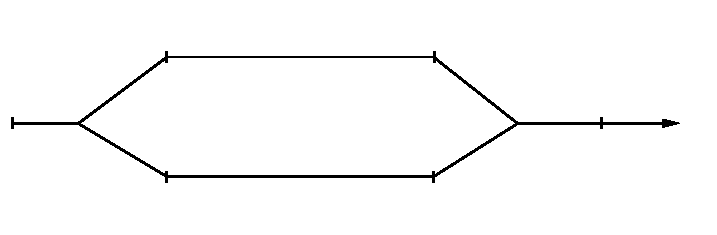
\includegraphics[width=16cm]{fig00c.pdf}
  \caption{Secuencia temporal en una estructura centralizada}\label{fig1es}
\end{figure}

Utilizando el enfoque de primer orden y los equivalentes ciertos, se obtiene:
\begin{eqnarray*}
b^C&=&\tau a-z_1\\
B^C&=&\psi_1t_1+\psi_{12}\bar{t}_2-\phi_1\\
D^C&=&\psi_2t_2+\psi_{12}\bar{t}_1-\phi_2
\end{eqnarray*}
y los niveles de esfuerzo de segundo \'optimo son:
\begin{eqnarray}
a^{C}&=&\frac{b+z_1}{\tau}\label{asoes}\\
t_1^{C}&=&\frac{(B+\phi_1)\psi_2-(D+\phi_2)\psi_{12}}{\psi_1\psi_2-\psi_{12}^2}\label{t1soes}\\
t_2^{C}&=&\frac{(D+\phi_2)\psi_1-(B+\phi_1)\psi_{12}}{\psi_1\psi_2-\psi_{12}^2}\label{t2soes}
\end{eqnarray}

Suponiendo perturbaciones independientes ($\sigma_{12}=0$), las intensidades \'optimas de los incentivos son:
\begin{eqnarray}
b^C&=&\frac{1}{\lambda(1+\rho\sigma_1^2\tau)}\label{bsoes}\\
B^C&=&\frac{\psi_2-\psi_{12}(1-\lambda D^C)}{\lambda[\psi_2+\eta\sigma_1^2(\psi_1\psi_2-\psi_{12}^2)]}\label{Bso1es}\\
D^C&=&\frac{\psi_1-\psi_{12}(1-\lambda B^C)}{\lambda[\psi_1+\eta\sigma_2^2(\psi_1\psi_2-\psi_{12}^2)]}\label{Dso1es}
\end{eqnarray}
Resolviendo conjuntamente para $B^C$ y $D^C$:
\begin{eqnarray}
B^C&=&\frac{1+\eta\sigma_2^2(\psi_2-\psi_{12})}{\lambda[1+\sigma_1^2\sigma_2^2\eta^2(\psi_1\psi_2-\psi_{12}^2)+\eta(\sigma_1^2\psi_1+\sigma_2^2\psi_2)]}\label{Bso2es}\\
D^C&=&\frac{1+\eta\sigma_1^2(\psi_1-\psi_{12})}{\lambda[1+\sigma_1^2\sigma_2^2\eta^2(\psi_1\psi_2-\psi_{12}^2)+\eta(\sigma_1^2\psi_1+\sigma_2^2\psi_2)]}\label{Dso2es}
\end{eqnarray}

De la soluci\'on centralizada se derivan varias conclusiones:
\begin{itemize}
\item A diferencia del caso de primer mejor, el contrato de segundo \'optimo no depende del componente altruista de los agentes.
\item Cuando las tareas del m\'edico son sustitutivas ($\psi_{12}>0$), las intensidades \'optimas de los incentivos sobre cantidad e intensidad se mueven conjuntamente.
\item Los incentivos son independientes entre agentes: modificar el par\'ametro de incentivos del hospital no altera los coeficientes \'optimos del contrato del m\'edico.
\item Cuando la intensidad se mide con mucho ruido y las tareas son casi sustitutivas, el contrato \'optimo tiende a debilitar o eliminar los incentivos del m\'edico y concentra una mayor parte del pago variable en el hospital.
\end{itemize}

\subsection{Estructura descentralizada}
Bajo descentralizaci\'on, el financiador contrata solo con el hospital y este dise\~na el contrato del m\'edico. El riesgo moral aparece, por tanto, tanto en la relaci\'on financiador-hospital como en la relaci\'on hospital-m\'edico. Resolviendo el juego por inducci\'on hacia atr\'as, primero caracterizamos el problema del hospital y despu\'es derivamos el contrato \'optimo del financiador. La secuencia de decisiones aparece en la Figura \ref{fig2es}.

\begin{figure}[htbp!]
  \centering
  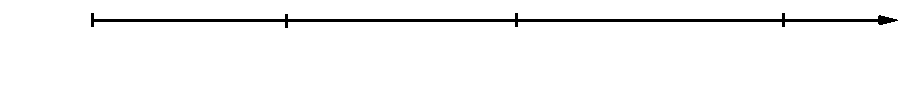
\includegraphics[width=15cm]{fig00d.pdf}
  \caption{Secuencia temporal en una estructura descentralizada}\label{fig2es}
\end{figure}

Utilizando los equivalentes ciertos correspondientes, el hospital resuelve:
\begin{eqnarray*}
\max\limits_{a,B,D}\ \mathbb{E}_{\bm{\epsilon}}[u_h]
&=&
f+(b-B)(a+t_1)+(d-D)t_2+z_1a-M\\
\nonumber \text{sujeto a }&&\\
t_1=t_1^{D}&=&\frac{(B+\phi_1)\psi_2-(D+\phi_2)\psi_{12}}{\psi_1\psi_2-\psi_{12}^2}\\
t_2=t_2^{D}&=&\frac{(D+\phi_2)\psi_1-(B+\phi_1)}{\psi_1\psi_2-\psi_{12}^2}\\
\hat{w}&=&\bar{w}
\end{eqnarray*}
donde $M$ recoge los costes de esfuerzo, la prima de riesgo del m\'edico y el componente fijo de su remuneraci\'on.

Sea $\theta=(\rho+\eta)$ y $\delta=\psi_1\psi_2-\psi_{12}^2$. Los pagos variables \'optimos al m\'edico son:
\begin{eqnarray*}
B^D&=&\frac{b(1+\sigma_1^2\rho\psi_1+\sigma_2^2\theta(\rho\delta\sigma_1^2+\psi_2))-d\eta\sigma_2^2\psi_{12}}{1+\psi_1\theta\sigma_1^2+\theta\sigma_2^2(\theta\delta\sigma_1^2+\psi_2)}\\
D^D&=&\frac{d(1+\sigma_2^2\rho\psi_2+\sigma_1^2\theta(\rho\delta\sigma_2^2+\psi_1))-b\eta\sigma_2^2\psi_{12}}{1+\psi_2\theta\sigma_2^2+\theta\sigma_1^2(\theta\delta\sigma_2^2+\psi_1)}
\end{eqnarray*}
Estas expresiones determinan los esfuerzos de equilibrio del m\'edico, $t_1(b,d)$ y $t_2(b,d)$, como funciones de los propios incentivos del hospital.

El problema del financiador es entonces:
\begin{eqnarray*}
\max\limits_{q,i,b,d}\ \mathbb{E}_{\bm{\epsilon}}[u_f]
&=&
a+t_1+t_2-\lambda\big(f+b(a+t_1)+dt_2\big)\\
a^D&=&\frac{b+z_1}{\tau}\\
t_1^D&=&t_1(b,d)\\
t_2^D&=&t_2(b,d)\\
\hat{b}&=&\bar{b}
\end{eqnarray*}

La soluci\'on general es algebraicamente compleja. Para el caso tratable en el que las tareas son independientes en la funci\'on de costes del m\'edico ($\psi_{12}=0$), pueden obtenerse expresiones cerradas para los incentivos y los esfuerzos. Lo relevante son sus implicaciones cualitativas. Igual que en la estructura centralizada, los par\'ametros altruistas no aparecen en los componentes variables \'optimos. Sin embargo, a diferencia del caso centralizado, los incentivos quedan conectados estrat\'egicamente entre niveles jer\'arquicos.

La comparaci\'on entre estructuras, en el caso de tareas independientes, muestra que el esfuerzo del hospital sobre cantidad es mayor bajo descentralizaci\'on, mientras que el esfuerzo del m\'edico sobre intensidad es menor. Que el esfuerzo del m\'edico sobre cantidad sea mayor bajo centralizaci\'on o bajo descentralizaci\'on depende de los costes marginales relativos de producir cantidad y de los par\'ametros de aversi\'on al riesgo. En t\'erminos m\'as generales, una vez que el hospital internaliza el problema de contrataci\'on aguas abajo, la estructura organizativa pasa a ser un determinante central de la asignaci\'on final del esfuerzo.

\section{Comparaci\'on de estructuras organizativas}
La soluci\'on descentralizada es lo bastante compleja como para que las est\'aticas comparadas limpias sean dif\'iciles de obtener en el caso general. Por ello conviene complementar los resultados anal\'iticos con ilustraciones num\'ericas. Nos centramos en dos cuestiones: c\'omo afecta la interacci\'on entre las tareas del m\'edico a incentivos y esfuerzo, y c\'omo modifican esos resultados los cambios en el ruido de las medidas de output.

\subsection{Cambios en la interacci\'on entre tareas}
La Figura \ref{fig3es} representa las intensidades \'optimas de los incentivos para una malla de valores de $\psi_{12}$ que va desde fuerte complementariedad hasta fuerte sustituibilidad.
\begin{figure}[htbp!]
  \centering
  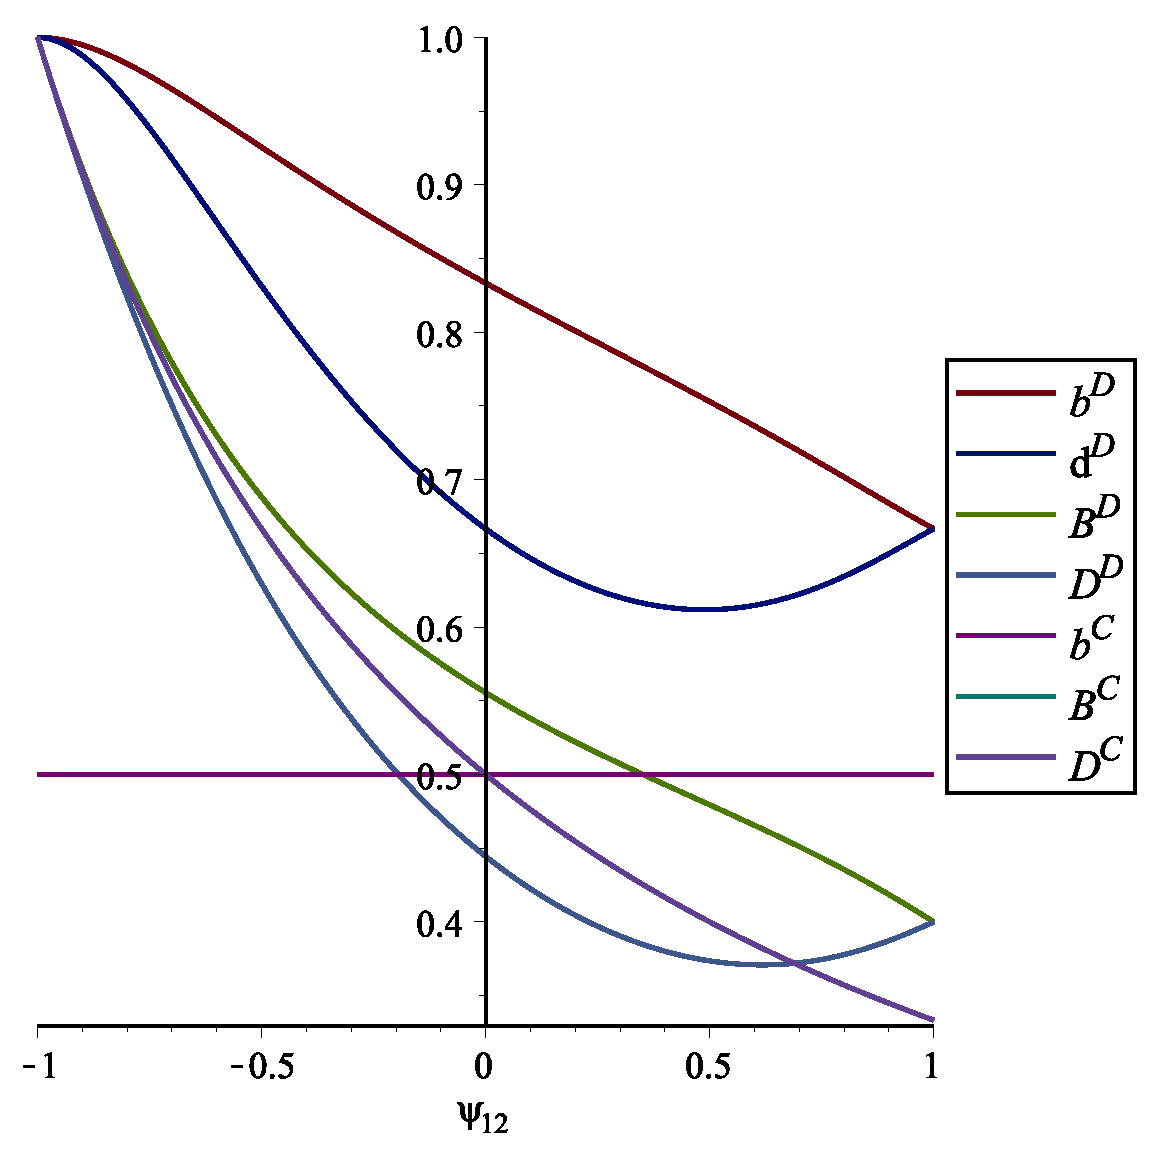
\includegraphics[width=8cm]{gr1-eps-converted-to.pdf}
  \caption{Incentivos \'optimos bajo estructuras descentralizada (D) y centralizada (C)}\label{fig3es}
\end{figure}

Salvo el incentivo constante del hospital sobre cantidad en la contrataci\'on centralizada, todos los pagos variables responden a la interacci\'on entre tareas del m\'edico. Cuando las tareas son fuertemente complementarias, los incentivos son altos y tienden a converger entre contratos. A medida que aumenta la sustituibilidad, los incentivos ligados a cantidad tienden a caer, mientras que los asociados a intensidad pueden aumentar a partir de cierto umbral. Un resultado especialmente interesante aparece cuando las tareas se aproximan a la sustituci\'on perfecta: bajo contrataci\'on centralizada, los incentivos del m\'edico colapsan hacia cero, mientras que bajo descentralizaci\'on el financiador sigue descansando en incentivos relativamente intensos transmitidos a trav\'es del contrato interno del hospital.

La Figura \ref{fig4es} traduce esos patrones de incentivos en diferencias de esfuerzo entre estructuras organizativas.
\begin{figure}[htbp!]
  \centering
  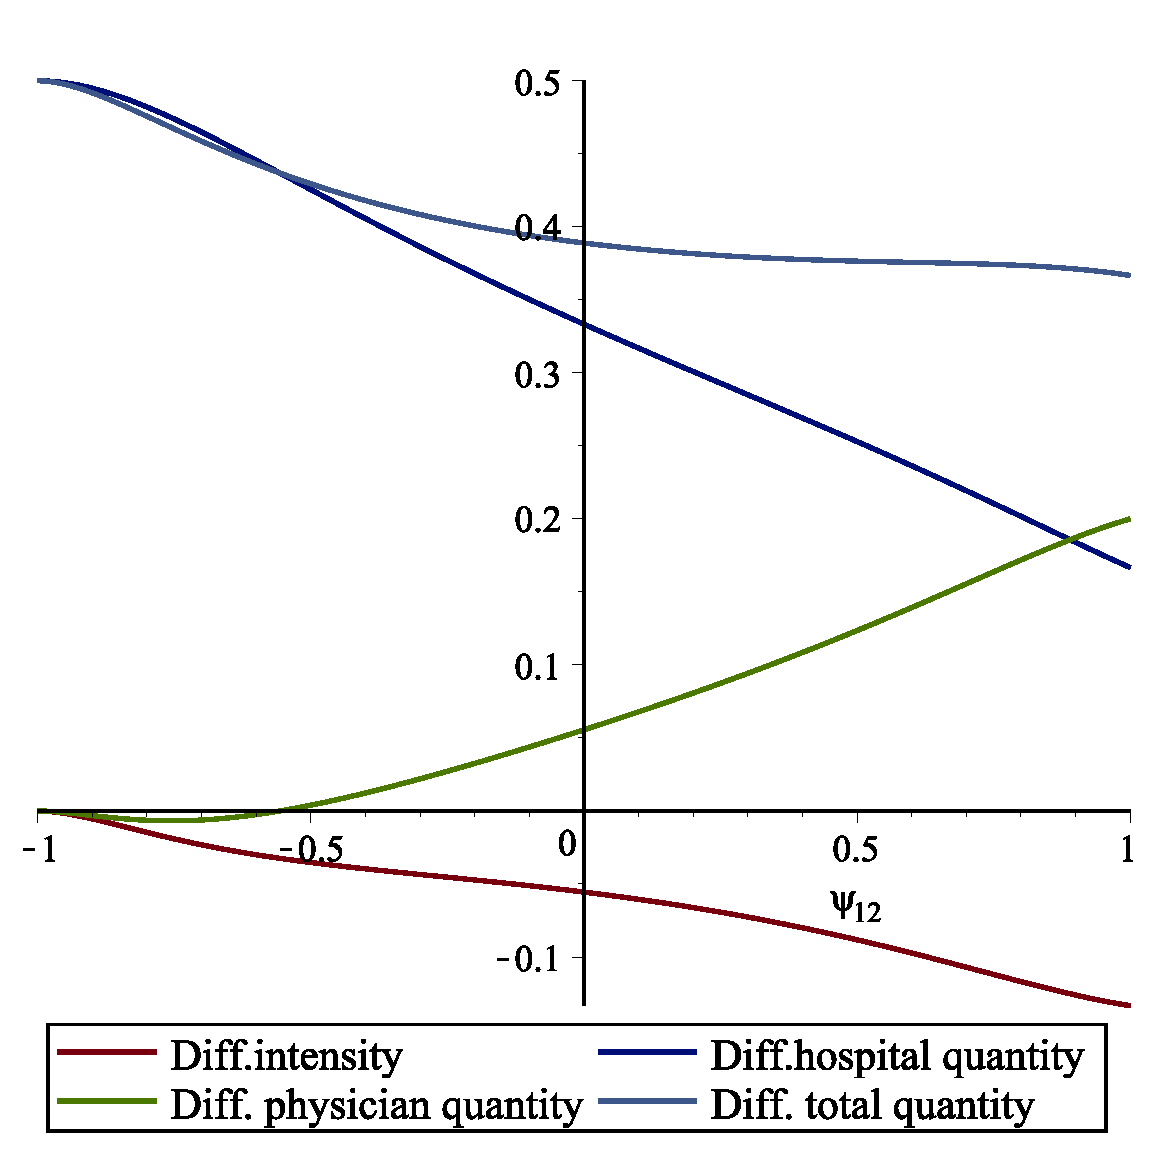
\includegraphics[width=8cm]{gr2-eps-converted-to.pdf}
  \caption{Diferencias de esfuerzo: descentralizada menos centralizada}\label{fig4es}
\end{figure}

El esfuerzo total sobre cantidad suele ser mayor cuando el principal contrata solo con el hospital. A medida que aumenta la sustituibilidad, la descentralizaci\'on desplaza los incentivos hacia la producci\'on de cantidad, mientras que la centralizaci\'on preserva incentivos relativamente m\'as fuertes para la intensidad. Cuando la cantidad se mide perfectamente ($\sigma_1=0$), ambas estructuras generan la misma cantidad total y alcanzan el primer mejor en esa dimensi\'on, aunque la intensidad sigue siendo menor bajo descentralizaci\'on. Cuando la intensidad se mide sin ruido ($\sigma_2=0$), ambas estructuras alcanzan el primer mejor en intensidad, pero la cantidad sigue siendo mayor bajo descentralizaci\'on.

\begin{figure}[htbp!]
  \centering
  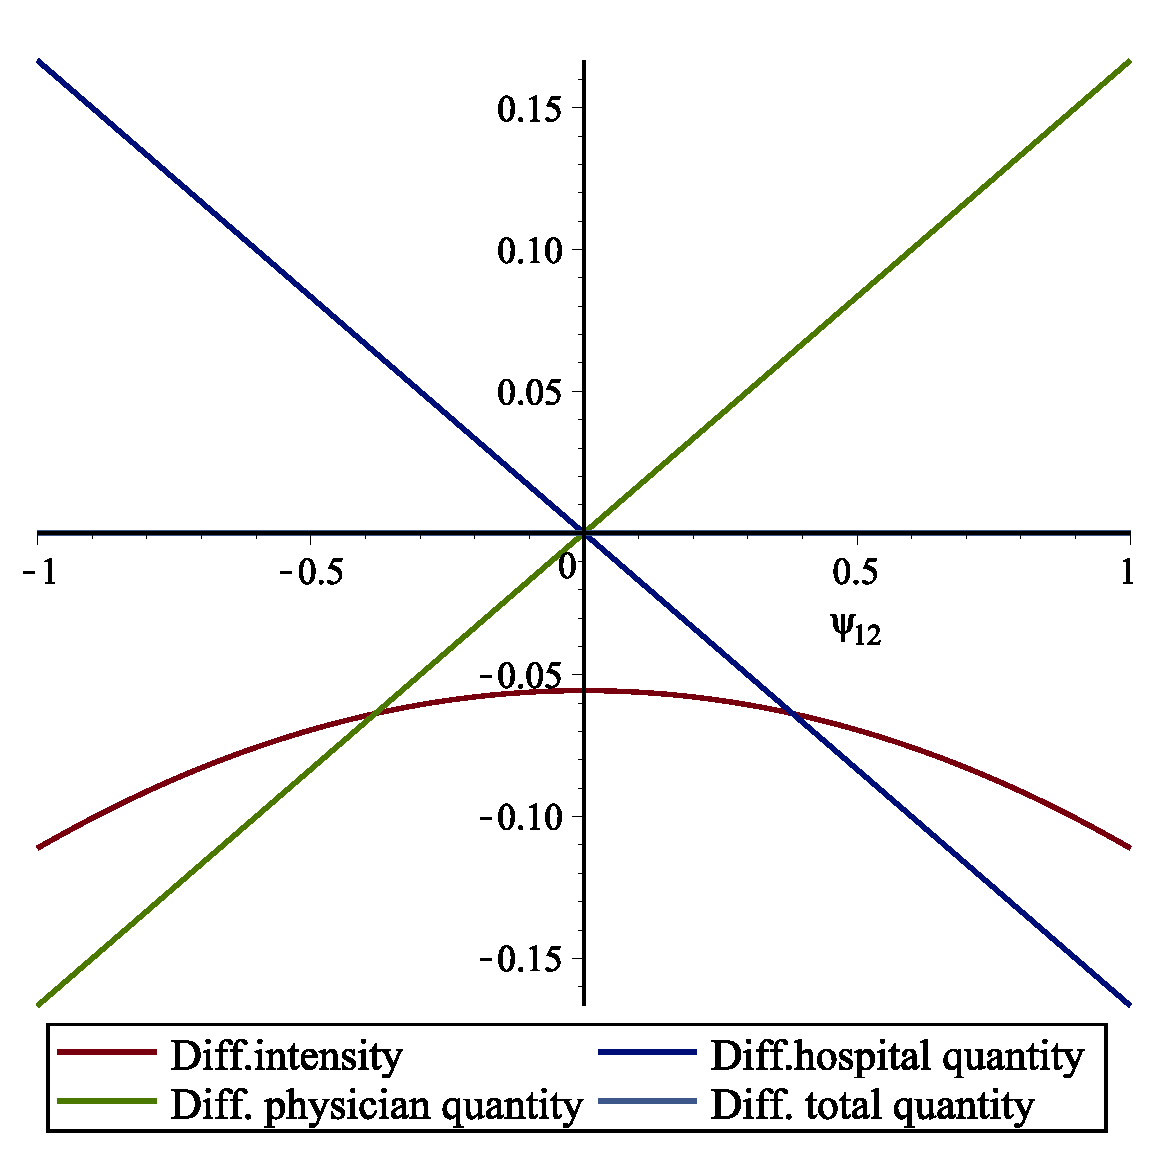
\includegraphics[width=8cm]{gr3-eps-converted-to.pdf}
  \caption{Diferencias de esfuerzo cuando $\sigma_1=0$}\label{fig5es}
\end{figure}

\begin{figure}[htbp!]
  \centering
  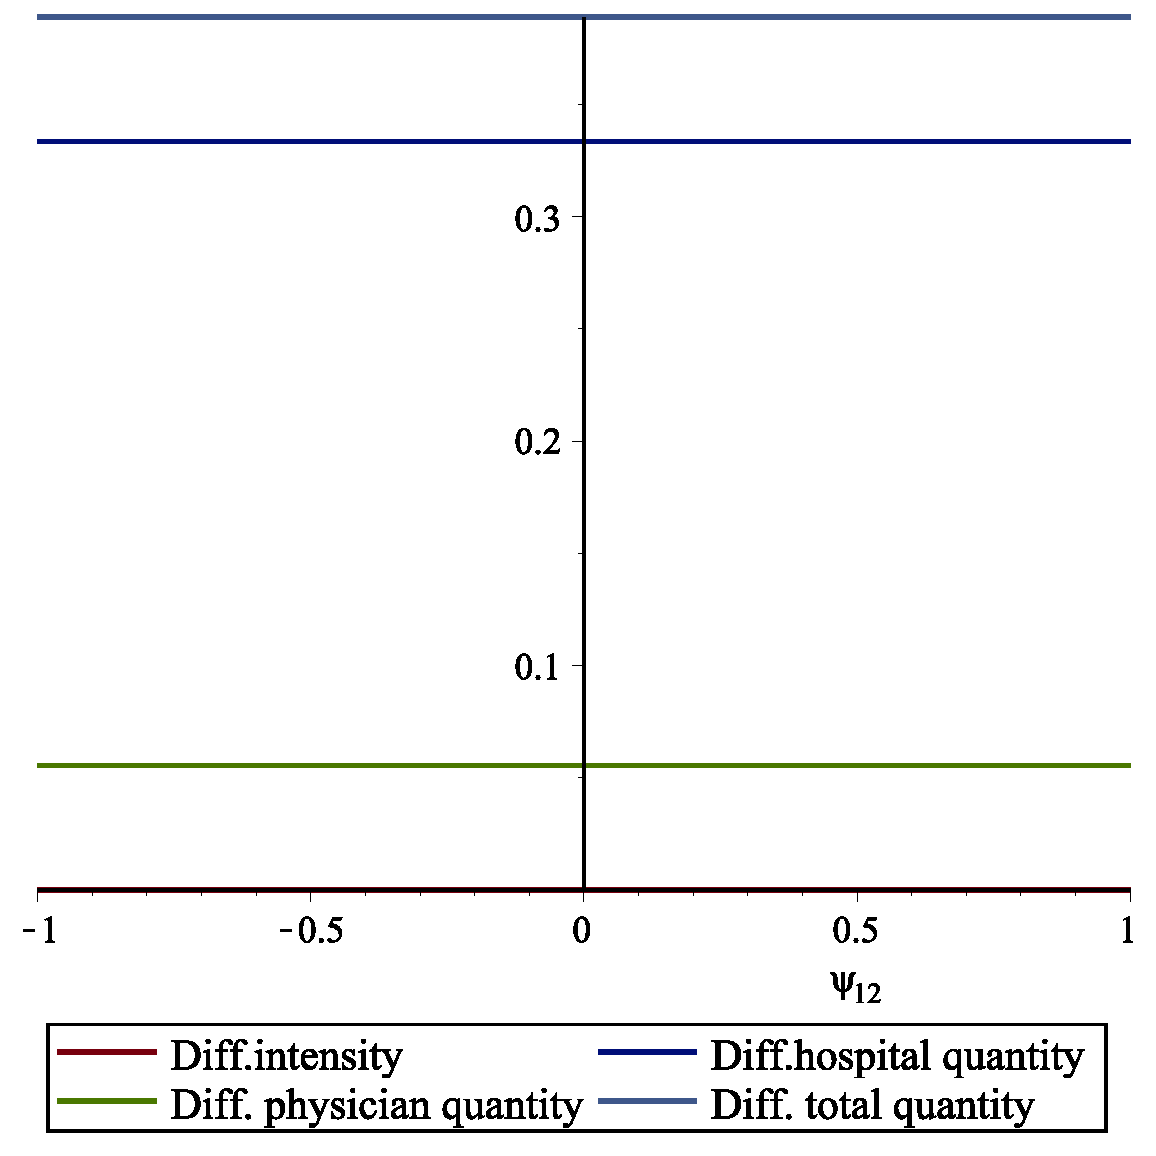
\includegraphics[width=8cm]{gr4-eps-converted-to.pdf}
  \caption{Diferencias de esfuerzo cuando $\sigma_2=0$}\label{fig6es}
\end{figure}

\subsection{Medici\'on imprecisa de los outputs}
Examinamos ahora c\'omo reaccionan los incentivos y los niveles de esfuerzo cuando las medidas de output se vuelven m\'as ruidosas para un valor fijo de $\psi_{12}$. La Figura \ref{fig7es} muestra el efecto de aumentar $\sigma_1$ cuando las tareas son sustitutivas de forma imperfecta ($\psi_{12}=0.5$).
\begin{figure}[htbp!]
  \centering
  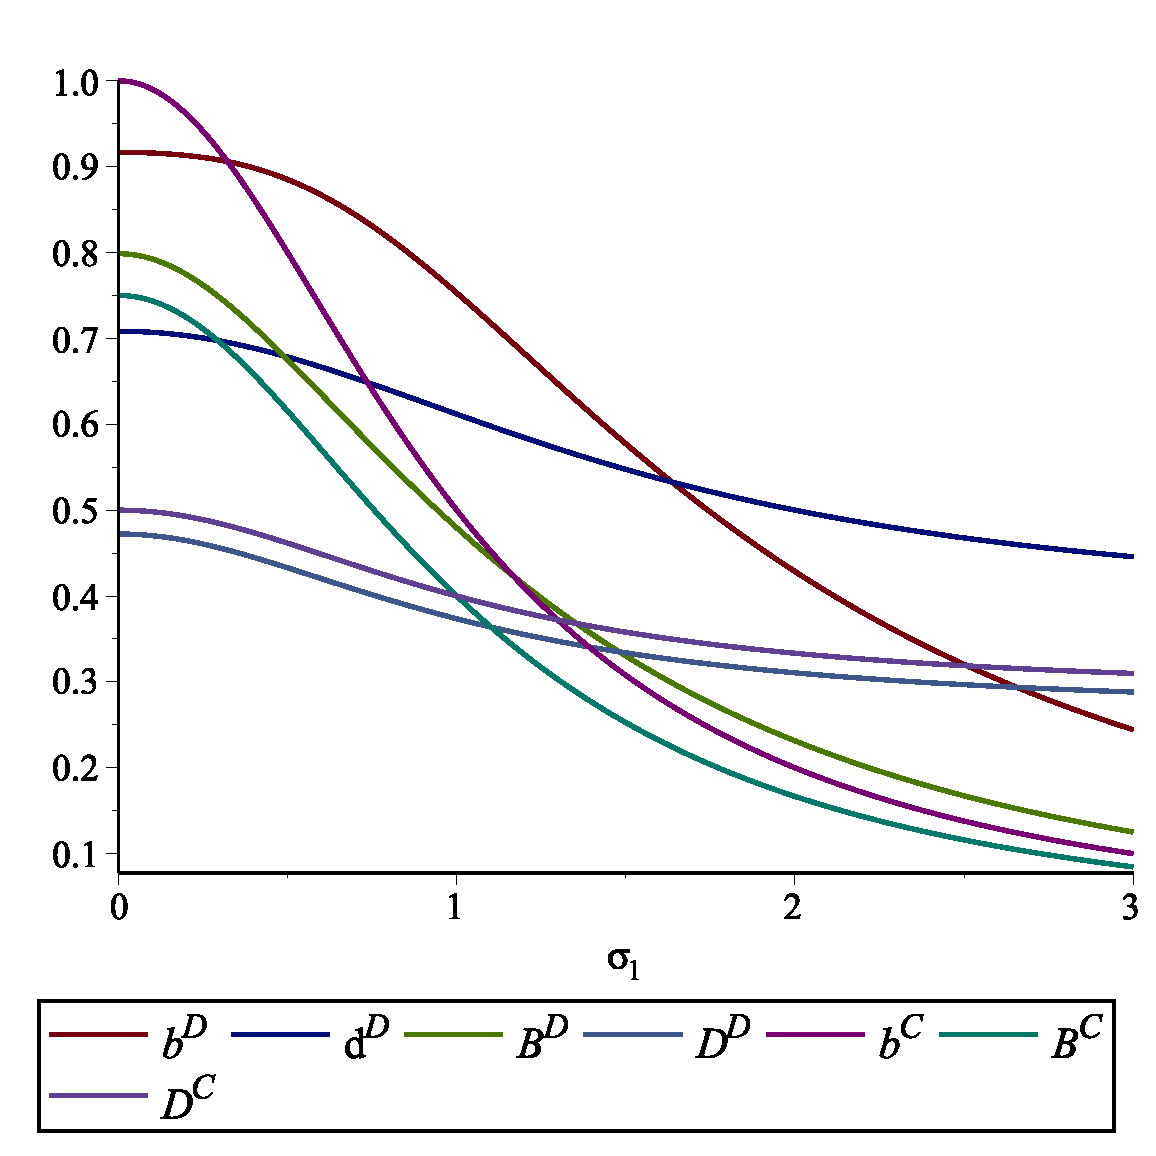
\includegraphics[width=8cm]{gr5-eps-converted-to.pdf}
  \caption{Incentivos \'optimos cuando aumenta $\sigma_1$}\label{fig7es}
\end{figure}

Todos los par\'ametros de incentivos disminuyen cuando la cantidad se mide con m\'as ruido. Los incentivos ligados a cantidad tienden a cero, mientras que los ligados a intensidad convergen a valores positivos. Las diferencias de esfuerzo asociadas se muestran en la Figura \ref{fig8es}.
\begin{figure}[htbp!]
  \centering
  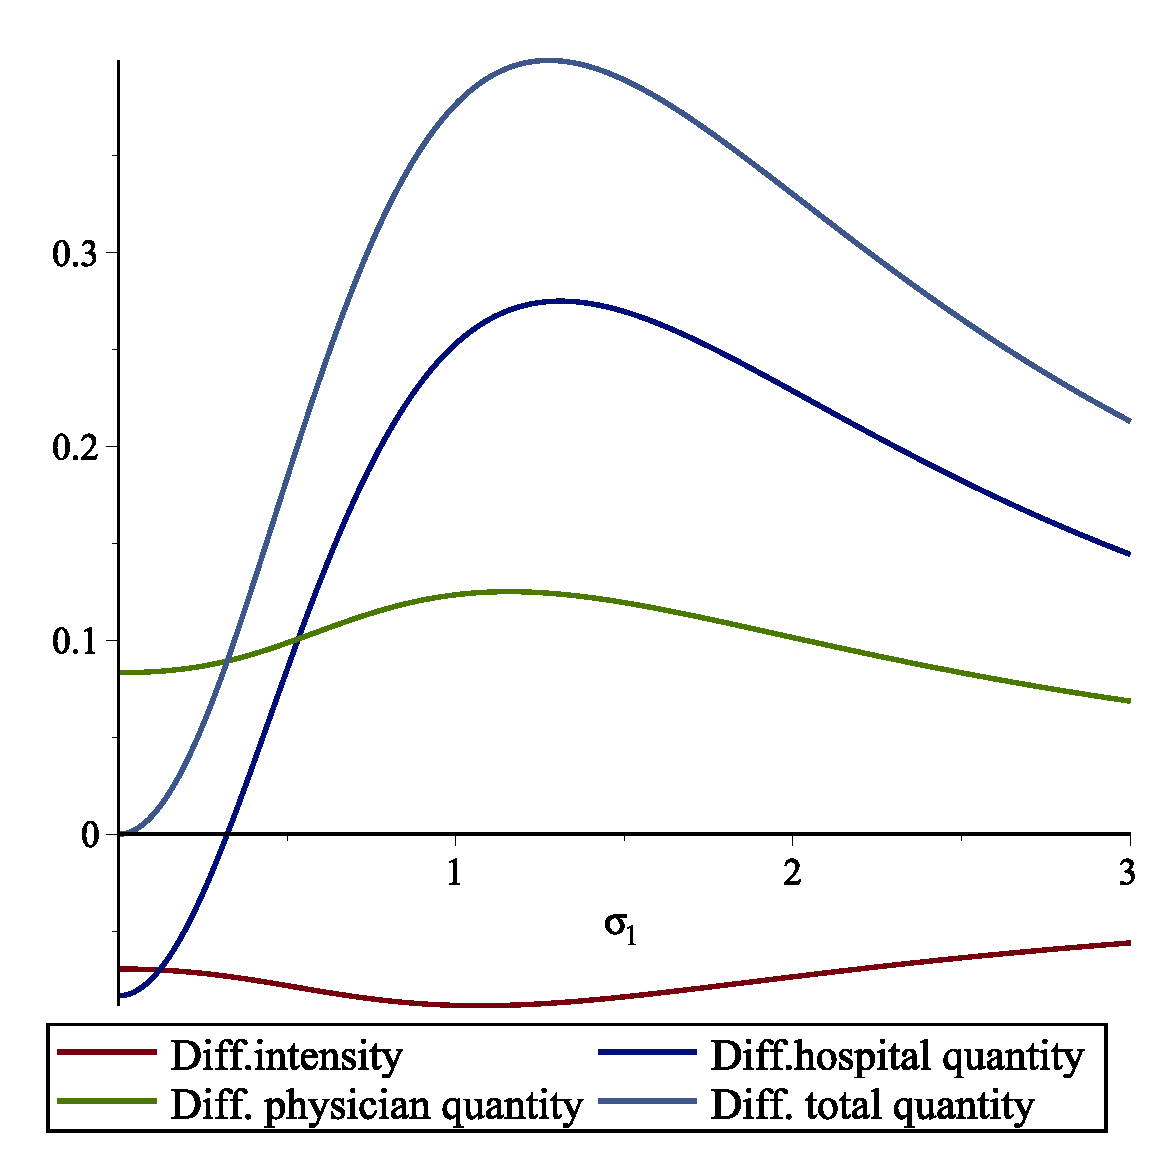
\includegraphics[width=8cm]{gr6-eps-converted-to.pdf}
  \caption{Diferencias de esfuerzo cuando aumenta $\sigma_1$}\label{fig8es}
\end{figure}

La intensidad sigue siendo mayor bajo centralizaci\'on, mientras que la cantidad total sigue siendo mayor bajo descentralizaci\'on. En el l\'imite, el esfuerzo del hospital sobre cantidad converge entre estructuras, pero el esfuerzo del m\'edico sobre cantidad permanece m\'as alto bajo descentralizaci\'on.

El ejercicio sim\'etrico puede realizarse para la varianza de la se\~nal de intensidad. La Figura \ref{fig9es} muestra que, a medida que aumenta $\sigma_2$, todos los incentivos vinculados a intensidad disminuyen hasta aproximarse a cero. Los incentivos sobre cantidad tambi\'en descienden, salvo el incentivo del hospital sobre cantidad en la estructura centralizada, que es independiente de $\sigma_2$.
\begin{figure}[htbp!]
  \centering
  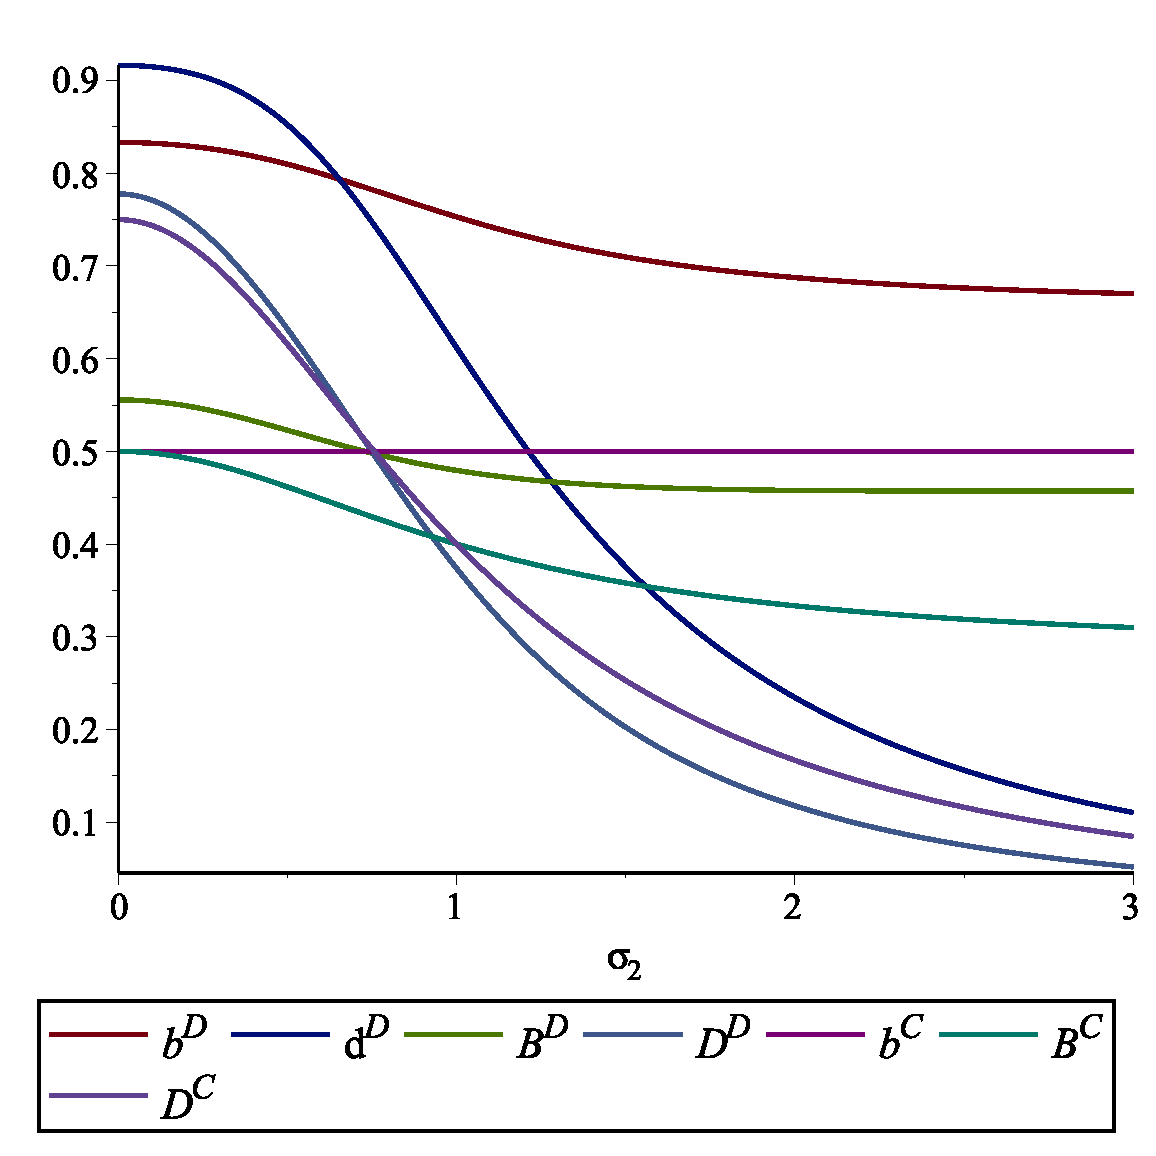
\includegraphics[width=8cm]{gr7-eps-converted-to.pdf}
  \caption{Incentivos \'optimos cuando aumenta $\sigma_2$}\label{fig9es}
\end{figure}

Las diferencias inducidas en el esfuerzo se resumen en las Figuras \ref{fig10es} y \ref{fig11es}.
\begin{figure}[htbp!]
  \centering
  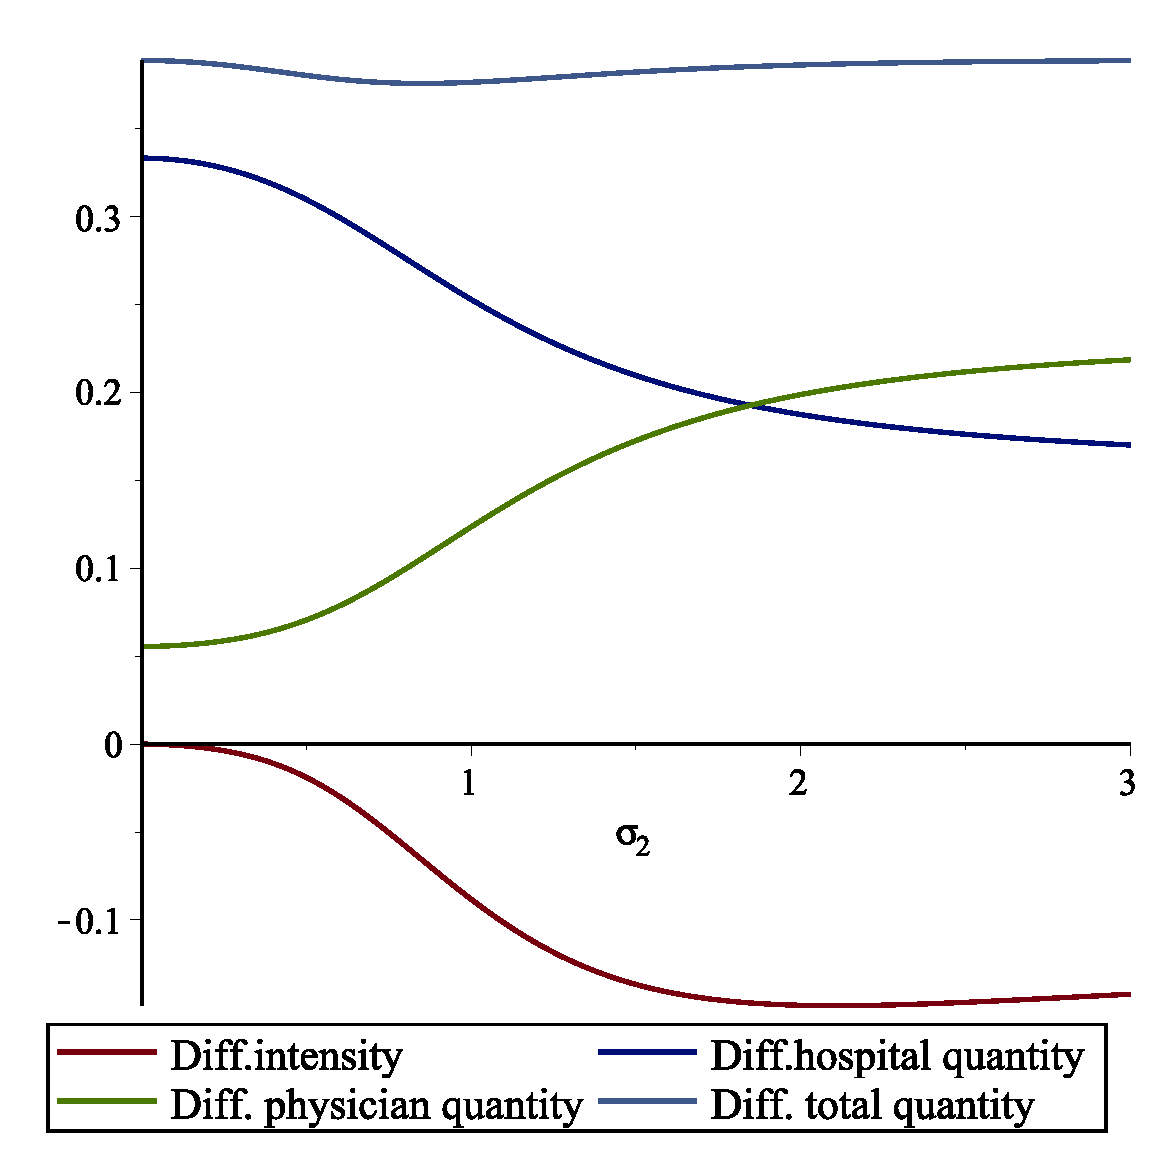
\includegraphics[width=8cm]{gr8-eps-converted-to.pdf}
  \caption{Diferencias de esfuerzo cuando aumenta $\sigma_2$ con tareas sustitutivas imperfectas ($\psi_{12}=0.5$)}\label{fig10es}
\end{figure}

\begin{figure}[htbp!]
  \centering
  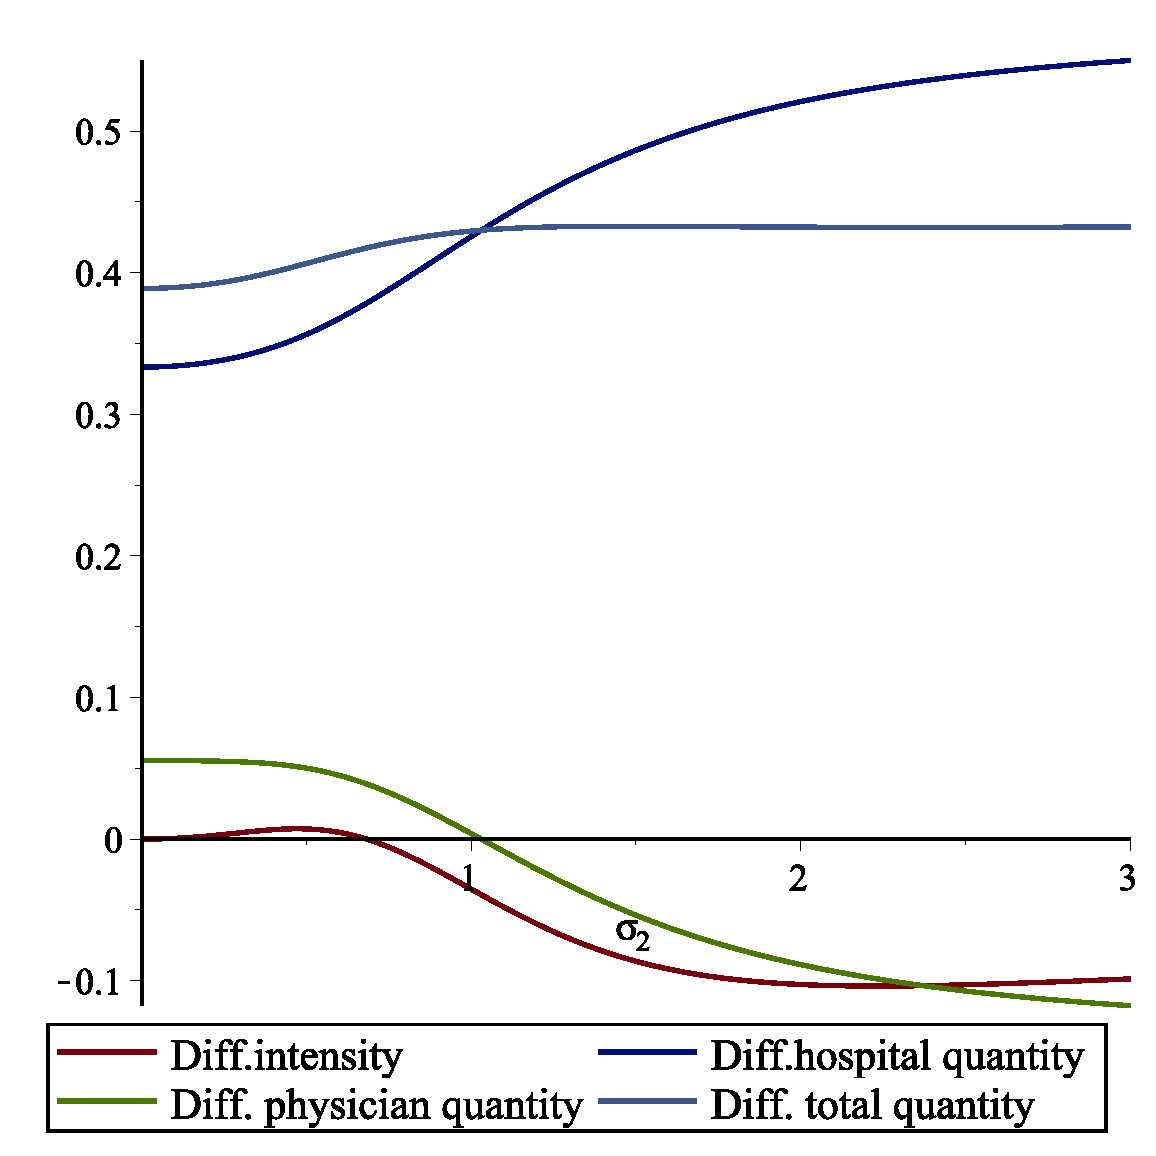
\includegraphics[width=8cm]{gr9-eps-converted-to.pdf}
  \caption{Diferencias de esfuerzo cuando aumenta $\sigma_2$ con tareas complementarias imperfectas ($\psi_{12}=-0.5$)}\label{fig11es}
\end{figure}

Con sustituibilidad imperfecta, la cantidad sigue siendo mayor bajo descentralizaci\'on, mientras que la intensidad sigue siendo mayor bajo centralizaci\'on. Con tareas complementarias, el patr\'on es m\'as matizado: para valores bajos de $\sigma_2$, la descentralizaci\'on puede dominar en cantidad e incluso en intensidad, pero a medida que crece el ruido la estructura centralizada pasa a dominar de forma creciente el desempe\~no del m\'edico.

\section{Conclusiones}
Este trabajo desarrolla un modelo de financiaci\'on hospitalaria con m\'ultiples agentes, m\'ultiples outputs y riesgo moral. El marco pone de relieve que la eficacia de los esquemas de incentivos depende no solo de los problemas de informaci\'on, sino tambi\'en de la arquitectura organizativa a trav\'es de la cual se implementan los contratos.

En el escenario de informaci\'on completa, el principal utiliza transferencias de suma fija, deja a los agentes en su utilidad de reserva y elige esfuerzos que igualan las condiciones marginales relevantes entre tareas y entre agentes. Bajo informaci\'on asim\'etrica, por el contrario, emergen contratos lineales de incentivos como resultado del equilibrio entre seguro y provisi\'on de esfuerzo.

La comparaci\'on entre contrataci\'on centralizada y descentralizada permite extraer tres conclusiones generales. En primer lugar, las motivaciones altruistas o vocacionales afectan a los niveles de esfuerzo en el benchmark de primer mejor, pero no alteran los componentes variables \'optimos de los contratos de segundo \'optimo. En segundo lugar, la estructura organizativa importa porque modifica la forma en que se internalizan los problemas de incentivos: en la contrataci\'on centralizada los incentivos son independientes entre agentes, mientras que bajo descentralizaci\'on quedan estrat\'egicamente conectados. En tercer lugar, el desempe\~no relativo de cada estructura depende tanto de la interacci\'on tecnol\'ogica entre tareas como del ruido en las medidas de output. En general, las estructuras centralizadas tienden a comportarse mejor en la dimensi\'on de intensidad, mientras que las estructuras descentralizadas inducen una mayor cantidad total.

Las simulaciones refuerzan esta idea. Cuando las tareas del m\'edico son muy sustitutivas, la contrataci\'on centralizada tiende a debilitar o eliminar los incentivos del m\'edico, mientras que la descentralizaci\'on preserva incentivos m\'as intensos a trav\'es del hospital. Cuando las medidas de output se vuelven m\'as ruidosas, las correspondientes intensidades de incentivos caen, pero la estructura organizativa sigue condicionando la direcci\'on de la reasignaci\'on del esfuerzo. La fuente concreta de la fricci\'on informativa, por tanto, no conduce mec\'anicamente a un dise\~no organizativo \'unico y preferible.

Estos resultados te\'oricos sugieren varias aplicaciones emp\'iricas. Una posibilidad es comparar resultados de eficiencia entre hospitales p\'ublicos, no lucrativos y con fines de lucro bajo distintos mecanismos de pago y arreglos organizativos. Otra es estimar c\'omo interact\'uan incentivos de baja y alta potencia con la autonom\'ia hospitalaria en datos de panel del sistema hospitalario espa\~nol.

\end{document}

